\begin{figure}[H]
  \centering
  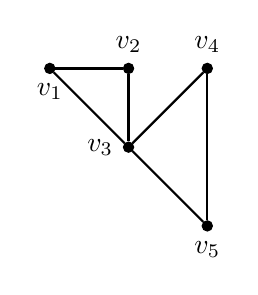
\begin{tikzpicture}
  \tikzset{enclosed/.style={draw, circle, inner sep=0pt, minimum size=.13cm, fill=black}}
  	\node[enclosed] at (0,2) (v1) [label=below:\(v_1\)] {};
    \node[enclosed] at (1,2) (v2) [label=above:\(v_2\)] {};
    \node[enclosed] at (1,1) (v3) [label=left:\(v_3\)] {};
    \node[enclosed] at (2,2) (v4) [label=above:\(v_4\)] {};
    \node[enclosed] at (2,0) (v5) [label=below:\(v_5\)] {};
    
	\path[thick] (v1) edge node {} (v2);
	\path[thick] (v1) edge node {} (v3);
	\path[thick] (v2) edge node {} (v3);
	\path[thick] (v4) edge node {} (v3);
	\path[thick] (v5) edge node {} (v3);   
	\path[thick] (v4) edge node {} (v5); 

  \end{tikzpicture}
  \caption{Ikke-orienteret, simpel graf til matrix.}
  \label{fig:stm}
\end{figure}